\documentclass{tudelft-report}

%% Set up the bibliography
\usepackage{biblatex}
\addbibresource{report.bib}

%% Additional packages and commands
\setlist{itemsep=-2pt} % Reducing white space in lists slightly
\renewcommand{\deg}{\si{\degree}\xspace} % Use \deg easily, everywhere

%% ----------------------------------------------------------------------
%%    Begin of document + Frontmatter (Roman page numbering)
%% ----------------------------------------------------------------------

\begin{document}

\frontmatter

%% Define the main parameters
\title{Deep Learning }
\subtitle{Come from dive into deep learning \\note For reading}
\author{我真的不懂忧郁}

\subject{} % Cover only
\affiliation{Delft University of Technology} % Cover only
\coverimage{figures/cover.jpg} % Aspect ratio of 2:3 (portrait) recommended
\definecolor{title}{HTML}{4884d6} % Color for cover title

\makecover

\begin{titlepage}

\begin{center}

%% Print the title
{\makeatletter
\largetitlestyle\fontsize{45}{45}\selectfont\@title
\makeatother}

%% Print the subtitle
{\makeatletter
\ifdefvoid{\@subtitle}{}{\bigskip\titlestyle\fontsize{20}{20}\selectfont\@subtitle}
\makeatother}

\bigskip
\bigskip

by

\bigskip
\bigskip

%% Print the name of the author
{\makeatletter
\largetitlestyle\fontsize{25}{25}\selectfont\@author
\makeatother}

\bigskip
\bigskip

%% Print table with names and student numbers
\setlength\extrarowheight{2pt}
\begin{tabular}{lc}
    Student Name & Student Number \\\midrule
    First Surname & 1234567 \\
\end{tabular}

\vfill

%% Print some more information at the bottom
\begin{tabular}{ll}
    Instructor: & I. Surname \\
    Teaching Assistant: & I. Surname \\
    Project Duration: & Month, Year - Month, Year \\
    Faculty: & Faculty of Aerospace Engineering, Delft
\end{tabular}

\bigskip
\bigskip

%% Add a source and description for the cover and optional attribution for the template
\begin{tabular}{p{15mm}p{10cm}}
    Cover: & Canadarm 2 Robotic Arm Grapples SpaceX Dragon by NASA under CC BY-NC 2.0 (Modified) \\
    % Feel free to remove the following attribution, it is not required - still appreciated :-)
    Style: & TU Delft Report Style, with modifications by Daan Zwaneveld
\end{tabular}

\end{center}

%% Insert the TU Delft logo at the bottom of the page
\begin{tikzpicture}[remember picture, overlay]
    \node[above=10mm] at (current page.south) {%
        
\includegraphics{figures/logo-black}
    };
\end{tikzpicture}

\end{titlepage}

\chapter*{Preface}
\addcontentsline{toc}{chapter}{Preface}

\emph{A preface...}

\begin{flushright}
{\makeatletter\itshape
    \@author \\
    Delft, \monthname{} \the\year{}
\makeatother}
\end{flushright}









\chapter*{Summary}
\addcontentsline{toc}{chapter}{Summary}

\emph{A summary...}


\tableofcontents
%\listoffigures
%\listoftables

\chapter*{Nomenclature}
\addcontentsline{toc}{chapter}{Nomenclature}

\emph{If a nomenclature is required, a simple template can be found below for convenience. Feel free to use, adapt or completely remove.}

\section*{Abbreviations}

\begin{longtable}{p{2.5cm}p{8cm}}
    \toprule
    Abbreviation & Definition \\
    \midrule\endhead % Add abbreviations alphabetically here:
    ISA & International Standard Atmosphere \\
    ... \\
    \bottomrule
\end{longtable}

\section*{Symbols}

\begin{longtable}{p{2.5cm}p{8cm}p{2.5cm}}
    \toprule
    Symbol & Definition & Unit \\
    \midrule\endhead % Add Latin symbols alphabetically here:
    $V$ & Velocity & [m/s] \\
    ... \\
    \midrule % Add Greek symbols alphabetically here:
    $\rho$ & Density & [kg/m$^3$] \\
    ... \\
    \bottomrule
\end{longtable}


%% ----------------------------------------------------------------------
%%    Mainmatter (Arabic page numbering)
%% ----------------------------------------------------------------------

\mainmatter
    \chapter{高斯网络概述}

\section{概述}

\begin{center}
    \begin{forest}
        forest scheme
        [PGM
            [Bayes Network(有向图模型)]
            [MarKov Network(无向图模型)]
            [Gaussian Network
                [Gaussian Bayes Network(有向图模型)]
                [MarKov Bayes Network(有向图模型)]
            ]
        ]
    \end{forest}
\end{center}

    
%% Prevent urls running into margins in bibliography
\setcounter{biburlnumpenalty}{7000}
\setcounter{biburllcpenalty}{7000}
\setcounter{biburlucpenalty}{7000}

%% Add bibliography
\printbibliography[heading=bibintoc,title=References]

%% ----------------------------------------------------------------------
%%    Appendix (Letters for chapters)
%% ----------------------------------------------------------------------

\appendix

\chapter{Source Code Example}
%\label{chapter:title}

\emph{Adding source code to your report/thesis is supported with the package {\normalfont\texttt{listings}}. An example can be found below. Files can be added using {\normalfont\texttt{\textbackslash lstinputlisting[language=<language>]\{<filename>\}}}.}

\begin{lstlisting}[language=Python]
"""
ISA Calculator: import the function, specify the height and it will return a
list in the following format: [Temperature,Density,Pressure,Speed of Sound].
Note that there is no check to see if the maximum altitude is reached.
"""

import math
g0 = 9.80665
R = 287.0
layer1 = [0, 288.15, 101325.0]
alt = [0,11000,20000,32000,47000,51000,71000,86000]
a = [-.0065,0,.0010,.0028,0,-.0028,-.0020]

def atmosphere(h):
    for i in range(0,len(alt)-1):
        if h >= alt[i]:
            layer0 = layer1[:]
            layer1[0] = min(h,alt[i+1])
            if a[i] != 0:
                layer1[1] = layer0[1] + a[i]*(layer1[0]-layer0[0])
                layer1[2] = layer0[2] * (layer1[1]/layer0[1])**(-g0/(a[i]*R))
            else:
                layer1[2] = layer0[2]*math.exp((-g0/(R*layer1[1]))*(layer1[0]-layer0[0]))
    return [layer1[1],layer1[2]/(R*layer1[1]),layer1[2],math.sqrt(1.4*R*layer1[1])]
\end{lstlisting}

\chapter{Task Division Example}
%\label{chapter:title}

\emph{If a task division is required, a simple template can be found below for convenience. Feel free to use, adapt or completely remove.}

\begin{table}[htb]
    \setlength\extrarowheight{4pt}
    \centering
    \caption{Distribution of the workload}
    \label{tab:taskdivision}
    \begin{tabularx}{\textwidth}{lXX}
        \toprule
        & Task & Student Name(s) \\
        \midrule
        & Summary & \\
        Chapter 1 & Introduction &  \\
        Chapter 2 &  & \\
        Chapter 3 &  & \\
        Chapter * &  & \\
        Chapter * & Conclusion &  \\
        \midrule
        & Editors & \\
        & CAD and Figures & \\
        & Document Design and Layout & \\
        \bottomrule
    \end{tabularx}
\end{table}

\chapter{Derivative of Vector}

\section{一元泰勒展开}

我们知道函数的一阶导数表示函数在一点的斜率,这意味着函数在这一点的斜率行为可以用一条切线逼近
\begin{equation}
    f(x)=f(x_0)+f'(x_0)(x-x_0)
\end{equation}

这可以看作是一个一元多项式,因此能够想到如果想更多描述函数在某点处的行为(比如描述函数斜率的变化率还需要知道二阶导数)可以用多项式去逼近,这就是泰勒开展
\begin{equation}
    f(x)=f(x_0)+f^{(1)}(x_0)(x-x_0)+\frac{f^{(2)}}{2!}(x-x_0)^2+\cdots+\frac{f^{(n)}}{n!}(x-x_0)^n+o((x-x_0)^{n+1})
\end{equation}

\section{二元泰勒展开}

定义点$(a_1,a_2)$在周边邻域的近似,泰勒定理需要研究的是在$(a_1,a_2)$周围邻域上的函数近似,设
$(x_1=a_1+tu,x_2=a_2+tv)$。构造辅助函数
\begin{equation}
    \Phi(t)=f(a_1+tu,a_2+tv)(0\leqslant t\leqslant 1)
\end{equation}

并把$\Phi$在$t=0$处展开去近似$t=1$的值
\begin{equation}
    \begin{aligned}
        & \Phi(t)=\Phi(0)+\frac{\Phi'(0)}{1!}t+\frac{\Phi''(0)}{2!}t^2+\cdots+\frac{\Phi^{(n)}(0)}{n!}t^n+\frac{\Phi^{(n+1)}(0)}{(n+1)!}t^{(n+1)}\\
        & \Phi(1)=\Phi(0)+\frac{\Phi'(0)}{1!}+\frac{\Phi''(0)}{2!}+\cdots+\frac{\Phi^{(n)}(0)}{n!}+\frac{\Phi^{(n+1)}(0)}{(n+1)!}\\
    \end{aligned}
\end{equation}

所以根据链式法则
\begin{equation}
    \begin{aligned}
        & \frac{df}{dt}=\frac{\partial f}{\partial x_1}\frac{\partial x_1}{\partial t}+\frac{\partial f}{\partial x_1}\frac{\partial x_2}{\partial t}\\
        & \Phi'(0)=u\frac{\partial f}{\partial x_1}(a_1,a_2)+v\frac{\partial f}{\partial x_2}(a_1,a_2)\\
        & \Phi''(0)=\cdots
    \end{aligned}
\end{equation}

令$t=1$,则$u=x_1-a_1,v=x_2-a_2$,因此得到二元函数的泰勒公式
\begin{equation}
    \begin{aligned}
        \Phi(1)=f(x_1,x_2)= &f(a_1,a_2)+(x_1-a_1)\frac{\partial f}{\partial x_1}(a_1,a_2)+(x_2-a_2)\frac{\partial f}{\partial x_2}(a_1,a_2) \\
        & +\frac{1}{2!} [(x_1-a_1)^2\frac{\partial^2 f}{\partial x_1^2}(a_1,a_2)+(x_1-a_1)(x_2-a_2)\frac{\partial^2 f}{\partial x_1\partial x_2}(a_1,a_2)\\
        & +(x_1-a_1)(x_2-a_2)\frac{\partial^2 f}{\partial x_2\partial x_1}(a_1,a_2)+(x_2-a_2)^2\frac{\partial^2 f}{\partial x_2^2}(a_1,a_2)]+\cdots
    \end{aligned}
\end{equation}

写成矩阵的形式,令$x=[x_1,x_2],a=[a_1,a_2]$

\begin{equation}
    f(x)=f(a)+\nabla f(a)\cdot (x-a)+\frac{1}{2}(x-a)^T H(a)(x-a)
\end{equation}

其中$H(a)$为二阶\textsl{Hessian}矩阵。

\begin{figure}[H]
    \centering
    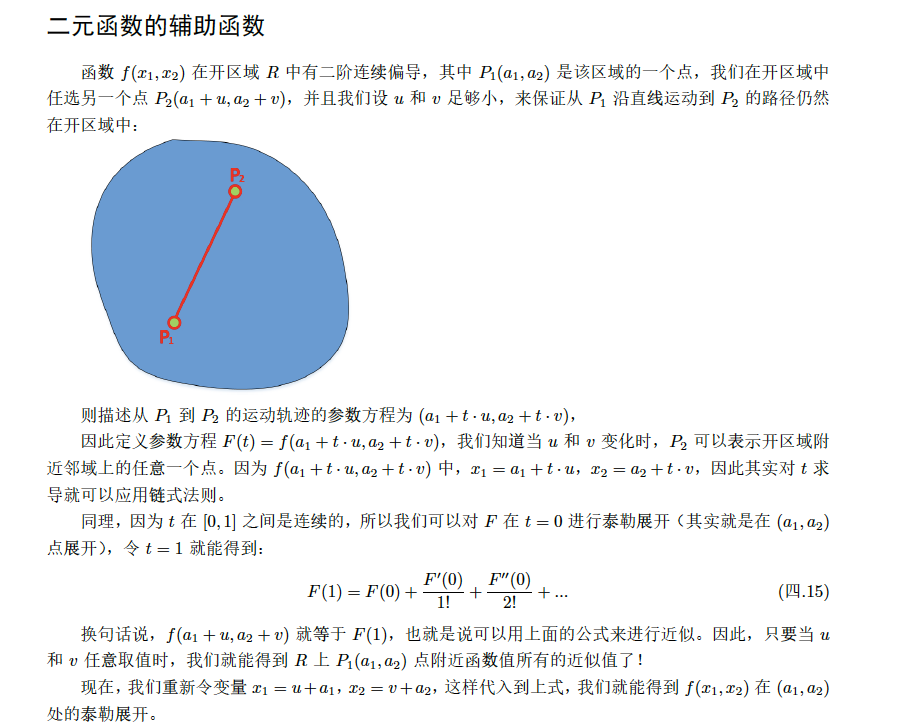
\includegraphics[scale=0.5]{figures/二元函数的辅助函数.png}
    \caption{二元函数的辅助函数}
\end{figure}

\section{小结}


函数在一点$a$展开,关注的是以$a$点附近邻域的函数的行为,肯定要满足在一点处的展开的值等于$a$处的函数值,所以泰勒级数中常数项等于$f(a)$,后面$n$阶导项等于$(x-a)^n$次方,当$x=a$时满足$f(x)=f(a)$。然后一阶导数项刚好用一条直线逼近。 % Create file to add

\end{document}
